\chapter{Поглощение света многослойной наночастицей} \label{chapt4}

\section{Введение}

Экстинкция электромагнитной волны, падающей на наночастицу,
определяется суммой рассеяния и поглощения этой же волны. Некоторые
аспекты управления рассеянием с помощью многослойных покрытий были
рассмотрены в предыдущей главе.  В настоящей главе будет рассмотрен
вопрос о фундаментальных ограничениях на эффективность поглощения
электромагнитного излучения уединённой наночастицей.

Ранее уже предпринимались попытки рассмотрения этого вопроса. В своей
работе~\cite{Tribelsky-2011} М.И. Трибельский показал, что существует
верхний предел, ограничивающий возможности поглощения для одного
мультиполя (моды). Коэффициенты Ми для поглощения электрическими
$\tilde{a}_n= {\rmfamily Re}\{a_n\} - |a_n|^2 $ и магнитными
$\tilde{b}_n= {\rmfamily Re}\{b_n\} - |b_n|^2 $ модами не могут
превысить значения $1/4$. Здесь $n=1$ соответствует случаю диполя,
$n=2$ квадрупольной моде, и так далее для б\'ольших значений $n$,
коэффициенты $a_n$ и $b_n$ имеют тот же смысл, что и в выражениях~\ref{eq:vector-harm1} и~\ref{eq:vector-harm2}.

Аналогичным образом, применяя только аналитические методы, Григорьев и
др.~\cite{Grigoriev-2015} рассмотрели эффект идеального поглощения на
примере двухслойной частицы, а именно случай диэлектрической сферы,
покрытой слоем золота или серебра. В дипольном приближении они
получили выражение для эффективного значения диэлектрической
проницаемости, обеспечивающего максимально достижимое поглощение в
сфере заданного размера.  В рамках теории эффективной среды
Максвелла-Гарнета ими было получено выражение для объёмной доли
диэлектрика, необходимой для возникновения эффекта идеального
поглощения в рассматриваемых двухслойных частицах.  Расчёт по этим
выражениям хорошо совпадает с вычислениями по уравнениям из работы
М.И. Трибельского~\cite{Tribelsky-2011} для случая $n=1$. Однако
указанный подход обладает рядом недостатков, среди которых можно
отметить ограниченную применимость (вследствие использования
дипольного приближения можно рассматривать только относительно
маленькие частицы) и то, что для большинства значений параметра
размера объёмная доля выражается комплексным числом.  Последний факт
делает эту теорию малопригодной для экспериментальной верификации.

Достоинством теории Ми является используемое разложение поля по
сферическим векторным гармоникам, что позволяет разделить вклад от электрической и магнитной дипольной моды, а также от квадруполей и мультиполей более высокого порядка. Таким образом,
становится возможен покомпонентный анализ спектрального отклика
многослойной сферы в зависимости от её дизайна. Например, в ряде
случаев удаётся совместить в спектре рассеяния положение нескольких
резонансов (электрических дипольного и квадрупольного). Это
создаёт эффект суперрассеяния~\cite{Fan-2010,Fan-2011}, когда
многослойная частица специального дизайна рассеивает сильнее, чем
однородная того же размера из произвольного изотропного
материала.

В данной главе рассматривается аналогичный эффект суперпоглощения,
когда из-за совмещения нескольких резонансов сечение поглощения
сферической наночастицы превышает фундаментальный предел для
мультиполя максимального порядка, возбуждённого в этой же частице.  В
этом случае, аналогично эффекту суперрассеяния, сечение поглощения
оказывается больше, чем у однородной частицы того же размера из
произвольного изотропного материала. Дело в том, что в случае
небольшой однородной сферы нет возможности совместить на одной
частоте, например, несколько электрических мод. Для заданного размера
сферы из одного материала различие в пространственной структуре низших
мод приводит к тому, что они оказываются существенно различны по
частоте. Моды высокого порядка могут оказаться разнесены по частотам
значительно меньше, чем ширина их полосы в спектре, однако такие
частицы оказываются гораздо больше, перестают быть наноразмерными и не
рассматриваются в настоящей работе. Аналогичным образом оказывается
невозможным совмещение на одной частоте нескольких магнитных мод.

Последнее возможное сочетание мод для случая однородной сферы, это
совмещение электрического и магнитного резонанса. Однако для
материалов, чаще всего используемых при изготовлении наночастиц,
положение низших электрических и магнитных мод, как правило, не
совпадает по частоте.  Впрочем, даже если и получится подобрать
сочетание материалов, размера наночастицы и используемой длины волны
(из-за наличия дисперсии необходимо задавать все
параметры модели с размерностью длины) так, что электрическая и
магнитная моды совпадут по частоте, то возможности совместить с ними
ещё одну моду не появится.  Чтобы это изменить, в систему необходимо
ввести дополнительные степени свободы, например, один или несколько
слоёв. Такая система и является объектом рассмотрения в
настоящей главе.

\section{Результаты оптимизации}

Для изучения поглощения электромагнитной плоской волны многослойными
наночастицами использовался тот же подход, который был применён в
предыдущей главе, посвящённой рассеивающим свойств.  А именно, с
помощью стохастической оптимизации были получены дизайны наночастиц,
обеспечивающие наилучшие рабочие характеристики; расчёт эффективности
поглощения основан на теории Ми. Такой подход оказался достаточно
универсальным. Он может быть применён для широкого класса материалов,
внешнего размера, произвольного (в пределах нескольких десятков) числа
слоёв наночастицы. Однако при проведении численной оптимизации всегда
существует ограничение по доступной вычислительной мощности, что
приводят к необходимости выбирать диапазон входных параметров
рассматриваемой модели. На начальном этапе были опробованы несколько
разных комбинаций используемых материалов и длин волн, выбран наиболее
перспективный с точки зрения возможных результатов вариант. В рамках
настоящей главы было принято решение ограничиться исследованием
поглощения света только трёхслойными частицы из заранее выбранных
материалов ($Si/Ag/Si$).  Использовались экспериментально измеренные
материальные параметры~\cite{palik-1997}. Большая часть результатов
была получена для длины волны $\lambda=500$~нм,
$\varepsilon_{\rmfamily Si} = 18.5 + i 0.63$,
$\varepsilon_{\rmfamily Ag} = -8.5 + i 0.76$, а в качестве параметров
оптимизации использовать толщины составных слоёв.

Целью исследования были структуры с максимальной эффективностью
поглощения $Q_{\rmfamily abs} = \alpha_{\mathrm abs}/\pi R^2$ для
заданной длины волны, где $\alpha_{\mathrm abs}$ это сечение поглощения,
а $R$ это внешний радиус наночастицы.  Результат оптимизации для
различных значений $R$ представлен на рисунках~\ref{img:q-abs}(а--в).
В данном случае, аналогично рисунку~\ref{img:min-max-min}(б), при
работе стохастического оптимизатора удалось получить очень хороший
уровень воспроизводимости получаемых результатов. В итоге, набор
дискретных значений полученных при оптимизации, сливается в сплошные
линии, изображённые на рисунке~\ref{img:q-abs}(а). На этом
рисунке дополнительными пунктирными линиями отмечены максимально
достижимые эффективности поглощения для дипольного ($n=1$) и
квадрупольного ($n=2$) резонансов, которые определяются
зависимостью~\cite{Tribelsky-2011}
\[Q^{(n)}_{\rmfamily abs\ max}=\frac{2n+1}{2q^2}\] через параметр
размера $q=2\pi R/\lambda$.  В рассматриваемой системе максимальный
порядок резонансного возбуждения мультиполей ограничен квадруполем
($n=2$). По сравнению с ним дизайны с внешним радиусом $R>60$~нм
демонстрируют большую эффективность поглощения, то есть выполняется условие
для режима суперпоглощения.

\begin{figure}[t]
  \begin{minipage}[ht]{0.495\linewidth}
    \centering{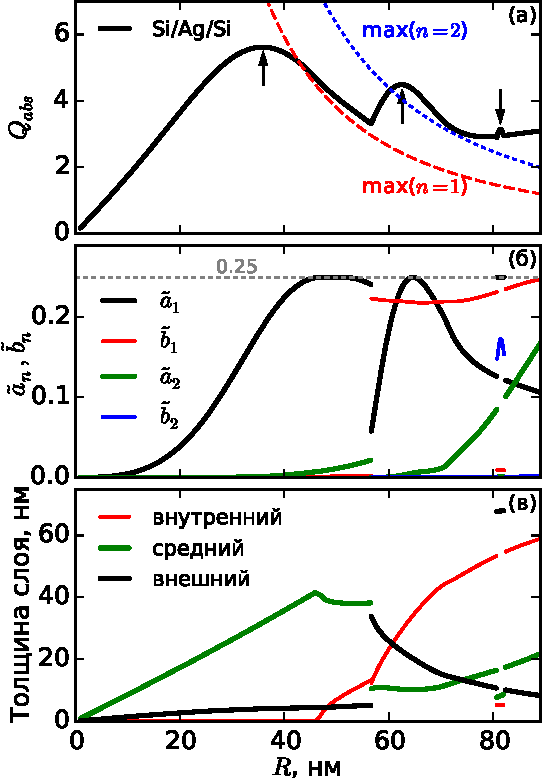
\includegraphics[height=1.35\linewidth]{2015-04-01-Qabs-SiAgSi-overview}}
  \end{minipage}
  \hfill
  \begin{minipage}[ht]{0.495\linewidth}
    \centering{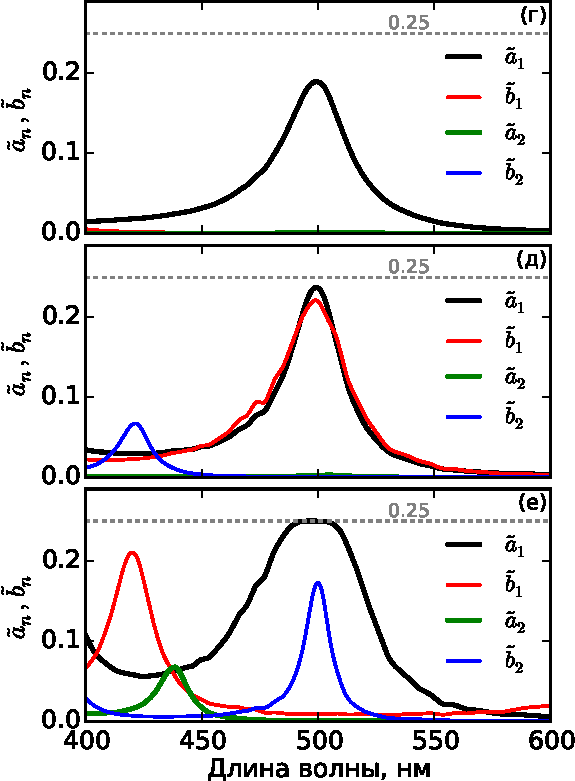
\includegraphics[height=1.35\linewidth]{2015-04-01-SiAgSi-ab-spectra4}}
  \end{minipage}
  \caption{ (а--в) Результат оптимизации эффективности поглощения
    $Si/Ag/Si$ наночастицей в зависимости от её внешнего радиуса, (а)
    эффективность поглощения, (б) коэффициенты поглощения в разложении
    Ми, где $\tilde{a}_1$ и $\tilde{a}_2$ относятся к электрическим, а
    $\tilde{b}_1$ и $\tilde{b}_2$ к магнитным диполю и квадруполю, (в)
    толщины составных слоёв наночастиц, (г--е) спектры коэффициентов
    поглощения в разложении Ми для дизайнов, соответствующих локальным
    максимумам на рисунке~\ref{img:q-abs}а.}
  \label{img:q-abs}  
\end{figure}


На рисунке~\ref{img:q-abs}(б) изображены значения коэффициентов Ми для
поглощения различными модами, горизонтальной пунктирной линией
отмечено значение теоретически достижимого предела, равное 1/4. В
случае небольшого размера оптимизированной частицы основной вклад в
поглощение даёт электрический диполь $\tilde{a}_1$.  Для дизайнов с
$R > 56.6$~нм оказалось, что использование одновременно электрического
и магнитного диполей позволяют достичь большего общего сечения
поглощения, чем в случае только с электрическим
диполем. Такое качественное изменение соответствует разрывам линий на
рисунках~\ref{img:q-abs}(б--в) и реализует режим суперпоглощения.
Необходимо отметить, что для небольшого диапазона размеров частицы
$80.7<R<82.1$~нм оптимальное поглощение обеспечивает использование
электрического дипольного $\tilde{a}_1$ и магнитного квадрупольного
$\tilde{b}_2$ резонансов, что приводит ещё к двум разрывам линий на
рисунках для соответствующих значений внешнего радиуса~$R$.

На рисунке~\ref{img:q-abs}(в) представлены толщины составных слоёв
наночастицы, полученные в результате оптимизации эффективности
поглощения.  Неожиданно оказалось, что дизайны с преобладающим
дипольным механизмом поглощения (т.е. для размеров частицы менее
56.6~нм) могут быть двух видов.  Чтобы получить наилучшее поглощение
для $R<46$~нм, хватает использования всего двух слоёв, при оптимизации
толщина внутреннего слоя исходного трёхслойного дизайна обратилась в
ноль.  При $R=46$~нм поглощение диполем почти достигает своего
теоретического предела ($\tilde{a}_1>0.249$), чтобы удерживать его
вблизи этого значения для больших значений $R$, оптимизатор начинает
наращивать толщину внутреннего кремниевого слоя.  В свою очередь, это
приводит к появлению слабого поглощения  $\tilde{a}_2$,
что, впрочем, не позволяет достичь режима суперпоглощения для $n=2$.

Для расчёта спектров на рисунках~\ref{img:q-abs}(г--е) были
использованы экспериментальные дисперсионные зависимости для
показателей преломления из работы\cite{palik-1997}. Спектры для
коэффициентов поглощения в разложении Ми построены для случаев,
соответствующих локальным максимумам на рисунке~\ref{img:q-abs}(а),
дополнительно отмеченных стрелками.  Спектр для дизайна с внешним
радиусом $R=36$~нм на рисунке~\ref{img:q-abs}(г) подтверждает
дипольный характер поглощения с резонансом на выбранной для
оптимизации длины волны $\lambda=500$~нм.  Спектры для дизайнов с
максимумами поглощения для $R=63$~нм и $R=81$~нм
(рисунки~\ref{img:q-abs}(д) и~\ref{img:q-abs}(е) соответственно)
обладают типичной для суперпоглощения структурой с вырождением
нескольких резонансов. На спектрах присутствуют дополнительные
резонансы, которые, впрочем, расположены в значительном отдалении от
выбранной для оптимизации длины волны и, соответственно, их вклад в
рассматриваемое поглощение мал.

Для спектра на рисунке~\ref{img:q-abs}(е) несколько неожиданной
оказалась форма кривой для электрической дипольной моды: вершина
резонансного колокола выглядит практически плоской.  Были проведены
дополнительные расчёты, построены спектры для коэффициентов Ми для
каждого слоя. Для рассматриваемой оптимизированной структуры
оказалось, что максимумы электрических дипольных резонансов,
сопоставляемые каждому слою, находятся на разных длинах волн, их
суперпозиция и приводит к соответствующему уширению спектра
поглощения.

Особо надо отметить, что для получения максимальной эффективности
поглощения вовсе не требуется режима суперпоглощения.  Из
рисунка~\ref{img:q-abs}(а) следует, что максимальная эффективность
соответствует малым размерам частицы, где значение коэффициента Ми для
поглощения заметно меньше теоретического предела.  Среди всех
рассмотренных структур двухслойная частица $Ag/Si$ с внешним радиусом
36~нм обладает максимальной эффективностью поглощения.  Для неё
сечение поглощения более чем 5 раз превысило её геометрическое
сечение, хотя значение коэффициента $\tilde{a}_1$ меньше
фундаментального предела приблизительно на 20\%.  Этот результат
хорошо согласуется с выводами работы~\cite{Miller-2014}, где
эффективность поглощения после нормировки на объём, оказалась
максимальной для частиц произвольной формы и небольшого размера с
преимущественным вкладом электрической дипольной моды.  Дополнительным
преимуществом двухслойных частиц может являться то, что они должны
быть проще и дешевле в производстве по сравнению с трёхслойными.  В то
же время для частиц большего размера ($R>60$~нм для рассмотренных
материалов) максимальная эффективность получается в режиме
суперпоглощения.  Это может оказаться существенно для случая, когда
изготовление многослойных частиц меньшего размера недоступно по
какой-либо технологической причине.

\begin{figure}[t]
  \centering{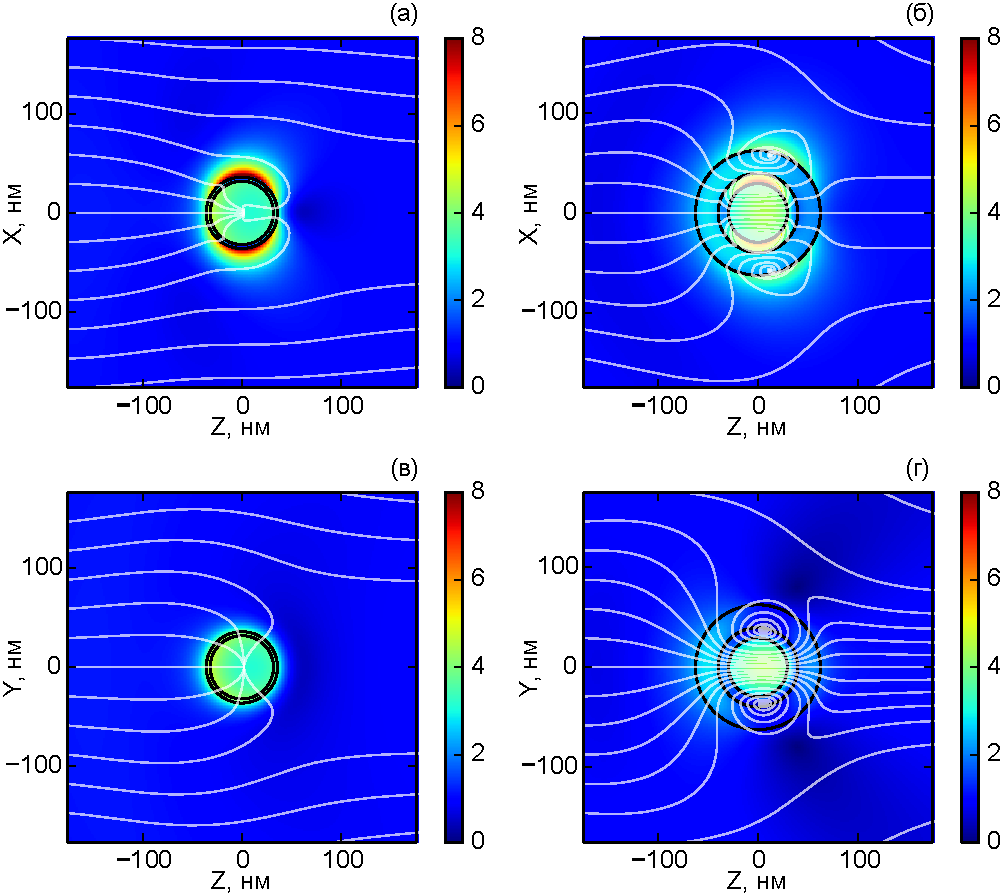
\includegraphics[width=0.95\linewidth]{SiAgSi-flow-YZ-Eabs-ru}}
  \caption{ Распределение амплитуды электрического поля нормированного
    на падающую волну для двух дизайнов, соответствующих локальным
    максимумам на рисунке~\ref{img:q-abs}а: (а,в) в режиме
    электрического диполя для $R=36$~нм и (б,г) в режиме
    суперпоглощения для $R=63$~нм. Распределения построены для (а,б)
    плоскости поляризации и (в,г) перпендикулярно к ней. Белые кривые
    обозначают линии потока энергии; плоская волна распространяется
    слева направо.}
  \label{img:absorb-field}
\end{figure}

Чтобы понять причину, по который частица меньшего размера может
обладать большой эффективностью необходимо рассмотреть картину
ближнего поля. На рисунке~\ref{img:absorb-field} построена амплитуда
электрического поля для случая большой и маленькой частицы.
Эффективность поглощения по определению
$Q_{\rmfamily abs} = \alpha_{\mathrm abs}/\pi R^2$ обратно
пропорциональна квадрату внешнего радиуса частицы, мощность поглощения
света наночастицами определяется как
\[
  P_{\mathrm {abs}}=\frac{1}{2}\int\sigma \left|E\right|^2dx\,dy\,dz,
\]
где локальная проводимость
$\sigma\propto \operatorname{\mathbb{I}m} (\epsilon)$ на выбранной
частоте падающего излучения слабо отличается у использованных
материалов ($Si$ и $Ag$). Так как интегрирование ведётся по объёму
частицы, то для обеспечения высокой эффективности оказывается важным
одновременный учёт двух факторов. Во-первых, необходимо использовать
резонансное поглощение с большим коэффициентом усиления
поля. Во-вторых, желательно обеспечить хорошее заполнение полем всего
материала частицы.

На рисунке~\ref{img:absorb-field}(а,в) хорошо видно, что для меньшей
частицы выполнены оба условия, по большей части её объёма коэффициент усиления поля падающей волны составляет приблизительно 3-4
раза. Частица большего размера на рисунке~\ref{img:absorb-field}(б,г)
демонстрирует приблизительно такое же усиление поля в центральной
части. В среднем слое усиление достигает более восьми раз, однако это
не позволяет компенсировать общее падение эффективности, вызванное
малой величиной поля во внешнем слое. В результате лучшую эффективность
поглощения демонстрирует меньшая частица, использующая только
электрическую дипольную моду.

Стоит отметить, что эта ситуация сохраняется в широком диапазоне длин
волн от 300 до 900~нм, для проверки была проведена серия оптимизаций с
шагом изменения длины волны 100~нм.  Что удивительно, некое
минимальное преимущество было получено для небольшой частицы даже для
длины волны $\lambda=300$~нм, где у серебра $\varepsilon$ оказывается
заметно больше единицы, а у кремния мнимая часть показателя становится
весьма значимой. При этом у оптимального дизайна основная часть поглощения
обусловлена электрической дипольной модой, а приблизительно 20\%
приходится на магнитную дипольную моду. Это наиболее заметное отличие
этого случая от других длин волн, где вклад в поглощение у мод,
отличных от электрической дипольной, пренебрежимо мал. Как уже
отмечалось, вывод об оптимальности небольшой частицы с преобладающей
электрической дипольной модой хорошо согласуется с аналогичными
выводами работы~\cite{Miller-2014}, в которой для расчёта
взаимодействия света с частицами использовался метод граничных
элементов (BEM) совместно с методом нелинейной оптимизации, основанном
на выпуклоотделимых консервативных приближениях (conservative convex
separable approximations), а в качестве материала для изготовления
наночастицы рассматривался ряд металлов, таких как $Al$, $Ag$, $Au$,
$Cu$, $Rh$ и $Os$.


Основной вопрос, который возникает при обсуждении данных,
представленных на рисунке~\ref{img:q-abs}, касается достоверности
полученных результатов.  В первой главе диссертации уже была
верифицирована программа расчёта по теории Ми, это позволяет
утверждать, что полученные дизайны действительно обладают заявленными
значениями эффективности поглощения.  Во второй главе был подробно
рассмотрен используемый алгоритм оптимизации, на ряде примеров была
показана его эффективность.  Так как она зависит от вида
оптимизируемой функции, то вопрос можно переформулировать следующим
образом: насколько можно доверять результатам оптимизации в случае
поиска максимального значения для функции эффективности поглощения
многослойной наночастицы в зависимости от толщины составных слоёв?

Сами по себе численные методы оптимизации не могут гарантировать, что
будет найден глобальный экстремум целевой функции. Они успешно
могут применяться для частичного решения задачи о существовании,
являясь способом нахождения новых дизайнов с заранее заданными
свойствами или близкими к ним.  Недостатком выбранного подхода является
отсутствие доказательства единственности полученного решения.  Другими
словами, оптимизатор может терять какие-то решения (точнее, не
находить их), нет гарантий, что получаемый ответ является глобальным и
единственным экстремумом.

При решении физических и инженерных задач можно опираться на косвенные
признаки, сопутствующие оптимальному решению.  В случае, если такое
решение вступает в противоречие с какими-то заключениями других
методов, применяемых для рассмотрения изучаемой системы, то возникает
возможность получить новое знание либо о самой системе, либо об
особенностях её рассмотрения с помощью стохастического
оптимизатора. Возможна и другая ситуация, когда оптимальное решение,
полученное численными методами, обладает набором свойств, которые
могут быть предсказаны при аналитическом рассмотрении или при
качественном анализе системы. В этом случае приходится признать, что
предсказательная способность выбранного численного метода ни в чём не
уступает другим теоретическим методам и в рамках использованных
допущений получаемые результаты являются достоверными. Рассмотрим с
этой точки зрения представленные на рисунке~\ref{img:q-abs}
результаты.

Как было отмечено выше, мощность поглощения света многослойными
сферическими наночастицами определяется квадратом амплитуды поля
внутри частицы.  Поэтому для получения максимального поглощения для
заданного внешнего размера в первую очередь выгодно изменять дизайн
наночастицы таким образом, чтобы возбуждение происходило с максимально
возможным усилением поля внутри частицы, то есть резонансным образом.
Знание о таком способе увеличения поглощения света наночастицей не
передавалось в оптимизатор, который искал наиболее подходящие дизайны
для фиксированного значения длины волны и внешнего радиуса сферы.
Другими словами, у оптимизатора не было возможности ориентироваться на
положение резонансов в спектре поглощения. Фиксирование значение длины
волны исключает возможность прямого получения спектральных
характеристик, фиксированный внешний радиус наночастицы исключает
возможность делать это косвенным образом, применяя преобразование
пространственного масштаба для уравнений Максвелла. Однако если
рассчитать для полученных дизайнов спектр зависимости коэффициентов
поглощения от длины волны, то оказывается, что условие резонансного
возбуждение выполняется как раз для оптимизируемой длины волны
$\lambda=500$~нм, что и отображено на рисунках~\ref{img:q-abs}~(г-е).  Это
свидетельствует о том, что с помощью численной оптимизации было
получено правильное решение.

Как уже отмечалось, в своей работе~\cite{Tribelsky-2011}
М.И. Трибельский показал что существует верхний предел, ограничивающий
возможности поглощения для одного мультиполя; коэффициенты Ми для
поглощения $\tilde{a}_n$ и $\tilde{b}_n$ не могут превысить $1/4$;
близкие к этой величине значения соответствуют резонансу, без которого
не получить высокой эффективности поглощения.  Метод численной
оптимизации не может провести подобный анализ.  Тем не менее когда
частица оказывается достаточно большой, чтобы в ней можно было
возбудить электрическую дипольную моду, то для оптимизированных
дизайнов один или несколько коэффициентов Ми для поглощения имеет
значение в интервале от~0.2 до~0.25.  Это ещё раз подтверждает
корректность выбранного подхода.

Для того чтобы лучше понять влияние мультипольных резонансов на
эффективность поглощения был выполнен дополнительный прогон
оптимизации. В нём искались дизайны, обладающие максимальным значением
величины $\tilde{a}_1$, являющуюся коэффициентом Ми для поглощения
электрической дипольной модой. На рисунке~\ref{img:q-abs-a1}
приводится сравнение двух прогонов оптимизации: (а--в) --- результаты,
соответствующие максимальному значению $Q_{abs}$ (полученного ранее),
(г--е) --- величине $\tilde{a}_1$.
\begin{figure}[t]
  \begin{minipage}[ht]{0.495\linewidth}
    \centering{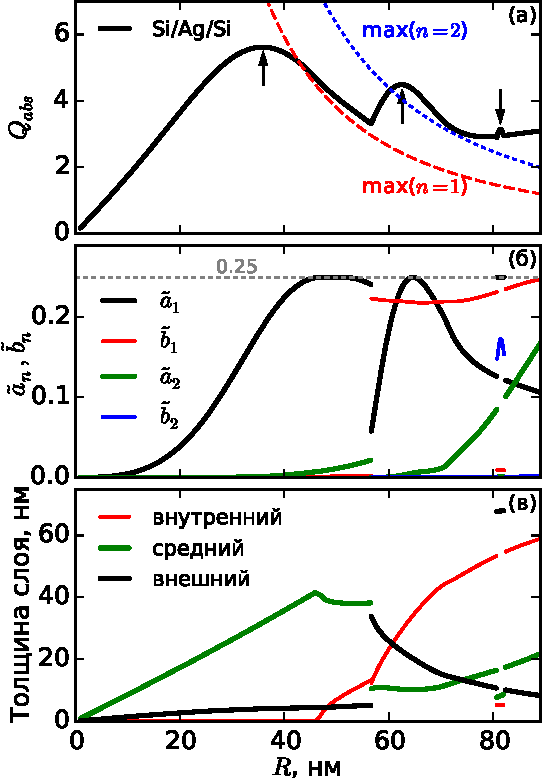
\includegraphics[width=0.95\linewidth]{2015-04-01-Qabs-SiAgSi-overview}}
  \end{minipage}
  \hfill
  \begin{minipage}[ht]{0.495\linewidth}
    \centering{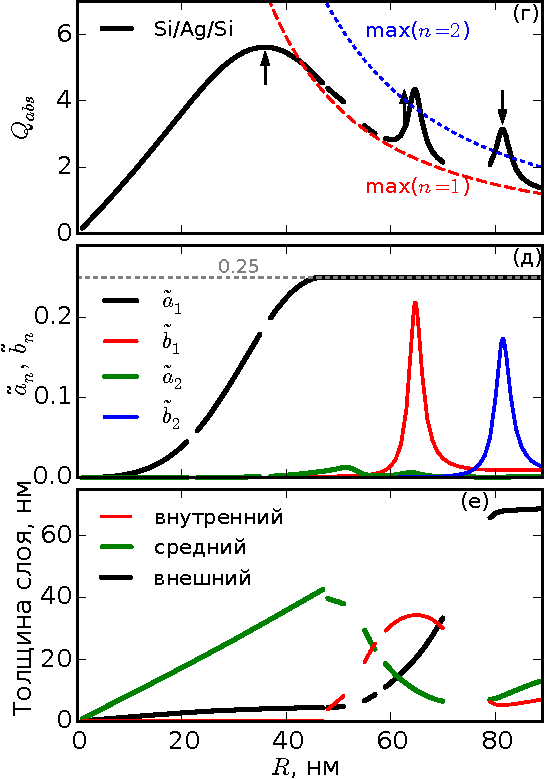
\includegraphics[width=0.95\linewidth]{overview-Qabs-a1-ru}}
  \end{minipage}
  \caption{ Результат оптимизации $Si/Ag/Si$ наночастицы в
    зависимости от её внешнего радиуса.  Копия
    рисунка~\ref{img:q-abs}(а--в), приводится для удобства сравнения
    оптимизации максимальной (а--в)~эффективности поглощения $Q_{abs}$
    и (г--е)~$\tilde{a}_1$, где (а,г)~эффективность
    поглощения, (б,д)~коэффициенты поглощения в разложении Ми, где
    $\tilde{a}_1$ и $\tilde{a}_2$ относятся к электрическим, а
    $\tilde{b}_1$ и $\tilde{b}_2$ к магнитным диполю и квадруполю,
    (в,е)~толщины составных слоёв наночастиц.}
  \label{img:q-abs-a1}
\end{figure}
Перед обсуждением полученных результатов необходимо сделать замечание
технического характера.  С одной стороны, для корректного сравнения
этих двух случаев хотелось бы ограничиться минимальным изменением
параметров моделирования.  Сам по себе расчёт эффективности поглощения
по теории Ми уже требует предварительного расчёта всех коэффициентов
разложения, поэтому изменение оптимизируемой функции оказывается
тривиальным.  С другой стороны, расчёт такой зависимости является
достаточно трудоёмким с вычислительной точки зрения.  Так как этот
прогон оптимизации приводится только в целях верификации предлагаемого
подхода, то был выбран значительно более крупный шаг изменения
внешнего радиуса наночастицы.  Для всех зависимостей на
рисунке~\ref{img:q-abs-a1} был использован один и тот же критерий для
определения мест разрывов, реализованной в виде программы для
построения графиков.  Применение этого критерия в случае крупного шага
изменения по горизонтальной оси привело к серии ложных срабатываний,
часть точек оказалась отделена от сплошной кривой с обеих сторон
разрывом и не отображается на графике.  Наиболее наглядно такая
ситуация представлена на рисунке~\ref{img:q-abs-a1}(е), где для
значений внешнего радиуса $70<R<78$~нм отсутствует визуализация данных
о толщинах составных слоёв.  Так как подобные пробелы отсутствуют при
построении коэффициентов Ми для наиболее интересного диапазона внешних
радиусов наночастицы и не влияют на общий характер демонстрируемой
зависимости, то было принято решение не тратить время на доработку
алгоритма построения графиков.  Принимая во внимание эту техническую
особенность, можно сравнивать случаи $Q_{abs}$
(рисунок~\ref{img:q-abs-a1}(а--в)) и $\tilde{a}_1$
(рисунок~\ref{img:q-abs-a1}(г--е)) при оптимизации дизайна наночастицы
для получения максимального значения этих величин.

Для небольших значений внешнего радиуса наночастицы $R<45$~нм оба
случая оптимизации демонстрируют идентичные результаты. Это выглядит
логично, так как в отсутствие других мультиполей эффективность
поглощения полностью определяется электрической дипольной
модой. Другими словами для этого диапазона размеров максимальное
значение $Q_{abs}$ соответствует максимальному значению
$\tilde{a}_1$. Небольшое расхождение возникает после появления
третьего слоя и в основном проявляется в дизайне наночастицы.
Существенное различие становится заметно после того, как $\tilde{a}_1$
на рисунке~\ref{img:q-abs-a1}(б) начинает уменьшаться, что
приблизительно соответствует общему размеру $R=55$~нм. На
рисунке~\ref{img:q-abs-a1}(д) $\tilde{a}_1$ продолжает держаться
вблизи значения $1/4$, а вот сопутствующее значение $Q_{abs}$
оказывается несколько меньше. Такое поведение в полной мере отражает
различие в выборе целевой функции для двух прогонов
оптимизации. Промежуточный результат можно сформулировать следующим
образом: даже в случае, когда поглощение происходит преимущественно на
дипольной моде, для получения максимальной эффективности поглощения
может быть выгодно иметь более сильную квадрупольную моду в ущерб
дипольной.

Интересно, что на рисунке~\ref{img:q-abs-a1}(д) при дальнейшем
увеличении внешнего размера оптимизированной наночастицы нарастают и
убывают вначале дипольная, а потом и квадрупольная магнитные моды. При
этом в точке максимума дипольной магнитной моды значение $Q_{abs}$
равно максимуму из первого прогона оптимизации для этого же внешнего
размера ($R=65$~нм), а дизайн наночастицы в этой точке совпадает у
обоих прогонов оптимизации на рисунке~\ref{img:q-abs-a1}.  Аналогичная
ситуация и вблизи максимума квадрупольной магнитной моды, где
совпадение наблюдается для диапазона $80.7<R<82.1$~нм.  Всё вместе это
ещё раз свидетельствует о верности выбранного подхода: результаты,
полученные при оптимизации с использованием разных целевых функций,
оказались согласованы между собой. 

Ранее в настоящей главе рассматривался вопрос о максимальной
эффективности поглощения у многослойной наночастицы для заданной длины
волны.  Использованный подход является достаточно общим, чтобы
его можно было применять для любой другой длины волны или некого
диапазона длин волн, например, для разработки дизайнов
спектрально-селективных поглотителей, работающих в нужной полосе
частот.  Более того, у предлагаемого подхода есть возможность
оптимизировать и другие параметры взаимодействия сферических
наночастиц со светом, востребованные в различных практических
приложениях.

Для демонстрации такой возможности была взята работа~\cite{Alu-2014},
авторы которой искали дизайны поглощающих частиц, обладающих малым
сечением рассеяния. В этой работе в качестве критерия эффективности
получаемых дизайнов использовалось отношение сечения поглощения к
сечению рассеяния $\eta_{\mathrm abs} = Q_{abs}/Q_{sca}$.  Для
сравнения был выбран случай, у которого значение сечения поглощения
$\alpha_{\mathrm abs}=\frac{3\lambda^2}{8\pi}$ для некого заданного
внешнего радиуса трёхслойной наночастицы.  При оптимизации изменялись
радиусы двух внутренних слоёв для получения максимального значения
эффективности.  Для значений относительной диэлектрической
проницаемости в слоях наночастицы $\epsilon_1 = 1.29+i0.01$,
$\epsilon_2 = -10.37+ i0.35$ и $\epsilon_3=8.4+i2.33$ был найден
дизайн с радиусами составных слоёв
$\{r_1, r_2, r_3\}=\{0.142,0.166,0.194\}\lambda$ и нормированной на
рассеяние эффективностью поглощения
$\eta_{\mathrm abs}^{(\alpha)} =7.65$.  Полученный дизайн с
преобладающим вкладом мод $a_1$ и $b_1$ хорошо согласуется с данными
работы~\cite{Alu-2014}, небольшое различие по сравнению с
эффективностью $\eta_{\mathrm abs}^{(\alpha)} =7.1$ из исходной работы
легко объяснимо.  При аналитическом подходе дизайн, обеспечивающий
наилучшую эффективность, получается из условия, согласующего
взаимодействие нескольких низших мод.  При численной оптимизации,
используемой автором диссертации, в расчёте по теории Ми учитываются
всё значимые моды.  В рассматриваемом примере небольшую поправку
внесли моды следующего порядка.

С помощью численной оптимизации появляется возможность получить
значительно большие значения $\eta_{\mathrm abs}$, для этого
необходимо, во-первых, доверить оптимизатору выбор внешнего радиуса и,
во-вторых, фиксировать не сечение поглощения, а его эффективность.
Если взять $Q_{\mathrm abs} = 5$, то оптимальный внешний радиус
оказывается значительно меньше, толщина внешнего слоя становится
равной нулю, радиусы двух других равны
$\{r_1, r_2\}=\{0.00635,0.00747\}\lambda$, а результирующее значение
$\eta_{\mathrm abs}^{(Q)} =544$.  Другими словами, такая небольшая
частица одновременно обладает сечением поглощения в 5 раз больше её
геометрического размера и очень большой нормированной на рассеяние
эффективностью поглощения. Этот результат хорошо демонстрирует, что
совместное применение численных и аналитических методов позволяет в
некоторых случаях получить дизайны со значительно большей
эффективностью по сравнению с исключительно аналитическим подходом.


\section{Выводы}

При совместном использовании метода стохастической оптимизации и
расчёта по теории Ми была исследована зависимость эффективности
поглощения падающей электромагнитной волны от размера
наночастицы. Было обнаружено, что в трёхслойных частицах $Si/Ag/Si$
возможно вырождение мультипольных резонансов, приводящее к эффекту
суперпоглощения, когда сечение поглощения оказывается больше, чем у
однородной частицы того же размера из произвольного изотропного
материала. Максимальная эффективность поглощения в рассматриваемой
системе была получена для небольших двухслойных частиц с преобладающей
ролью электрического дипольного резонанса. В серии дополнительных
оптимизаций была показана достоверность получаемых результатов.

\clearpage
